\section{Absolute detection efficiency of the NC\label{sec-nceff}}
%\subsection{Overview}
For the normalization of the neutron spectrum, the absolute detection efficiency of the NC is the most important one. In this section we evaluate the absolute efficiency with quasi-free $K^0$ production events. Note that the momentum dependence of the neutron reaction cross section is known to be almost flat in the region of interest as described in Sec. \ref{sec-geantnc}, and thus we do not consider the momentum dependence in the present analysis.
\subsection{$K^0_s$ quasi-free charge-exchange production}
We consider the $K^0_s$ charge-exchange production,
\begin{eqnarray}
K^- + ^3{\rm He} &\to& K^0_s + n + d_s \label{eq-chargeex} \\
	& &K^0_s \to \pi^+ +\pi^-,
\end{eqnarray}
where $d_s$ is a spectator deuteron. By detecting the $K^0_s$ with the CDS, the neutron trajectory can be obtained in terms of missing momentum, and thus we can obtain the neutron flux on the NC to evaluate the neutron detection efficiency. The momentum of the forward-going neutron in this reaction is about 1.1 GeV/$c$, which is close to the region of interest. Therefore, this procedure is suitable to evaluate the detection efficiency of the NC. %Note that the detection efficiency can be assumed to be flat in this momentum range. 

\subsection{$K^0_s$ selection in the CDS}
We analyzed the CDS data to obtain the $K^0_s$ event at first. Here the $K\otimes CDH2$ trigger data was used to avoid bias from the forward counters. Figure \ref{fig-k0select}(left) shows the reconstructed $\pi^+\pi^-$ invariant-mass spectrum, where the $K^0_s$ signal region was defined by $\pm2\sigma$ of the peak ( 0.485$<$IM($\pi^+\pi^-)<$0.512 ). By selecting the $K^0_s$ region, the missing-mass distribution of the $p(K^-,K^0_s)X$ was obtained as shown in Fig. \ref{fig-k0select}(right). In the figure, we can identify the missing neutron peak broadened by the Fermi motion in $^3$He. We selected the missing neutrons by $\pm2\sigma$ of the peak (0.80$<$MM$<$1.08 GeV/$c^2$). To evaluate the background distribution in the missing-mass distribution, we difined sideband regions in the $\pi^+\pi^-$ invariant mass; the left side is the region from 0.443 to 0.467 GeV/$c^2$, and the right one is from 0.524 to 0.548 GeV/$c^2$ as shown in Fig. \ref{fig-k0select}(left).

\begin{figure}[]
\begin{center}
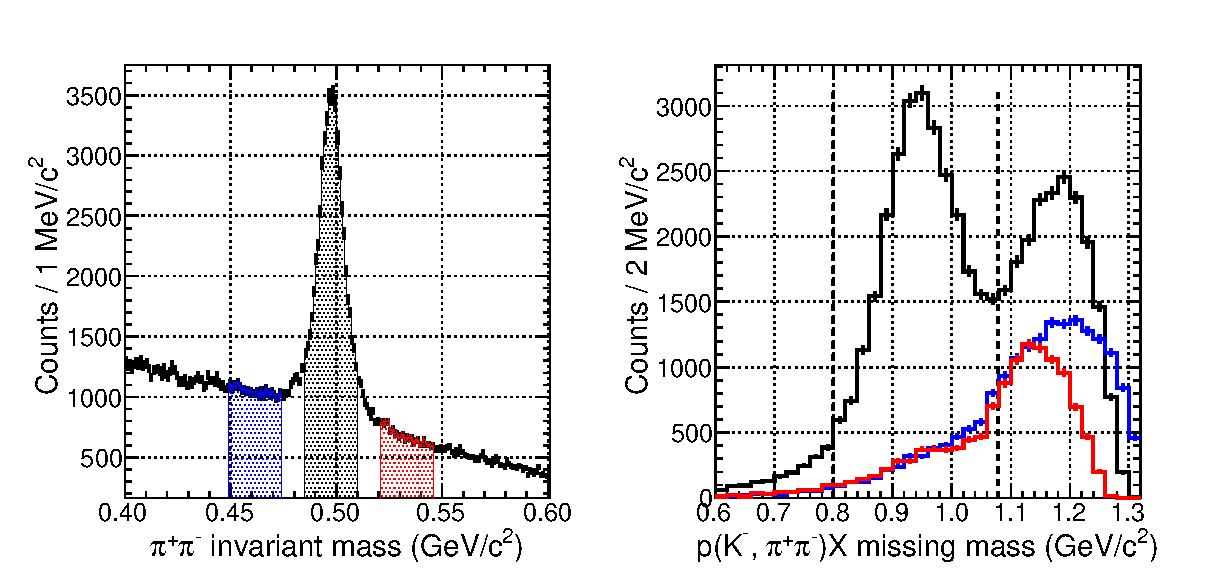
\includegraphics[width=\columnwidth]{./fig/k0-selectcut.eps}
\caption[$\pi^+\pi^-$ invariant-mass distribution and $(K^-,\pi^+\pi^-)X$ missing-mass distribution.]{(left)$\pi^+\pi^-$ invariant mass-distribution. The $K^0_s$ selection is shown with the black hatch, while sideband regions are defined as the blue and the red hatches. (right) $(K^-,\pi^+\pi^-)X$ missing-mass distribution assuming stopped proton target. The black histogram represents the $K^0_s$ events and the blue and the red histograms represent sideband events.}
\label{fig-k0select}
\end{center}
\end{figure}
\if0
\subsubsection{Event purification}
We have also employed rather tight cut conditions to check the systematics. One requires the hit numbers on IH and CDH to be 2 since the charge-exchange reaction emits only two charged particles via $K^0_s\to \pi^+\pi^-$ decay. The other one impose the $D^{helix}_{CA}$ and $D^{beam}_{CA}$ to be less than 2 cm in addition, namely we requested that the $K^0_s$ can define the vertex well.    
\fi
\subsubsection{Background evaluation}
To extract the signal of the quasi-free reaction (3.7) from the missing mass of the $p(K^-,K^0_s)X$, we evaluated the backgrounds which mainly consists of non-resonant background of $\pi^+\pi^-$, and pion associated reactions. The non-resonant background was obtained with the average of the sideband regions, and the pion associated reactions, such as $K^-p\to \pi^0K^0_sn$, were evaluated by the simulation. Figure \ref{fig-nceff1}(left) shows a typical decomposition of the $p(K^-,K^0_s)X$ missing-mass distribution.

\begin{figure}[]
\begin{minipage}{0.5\textwidth}
\begin{center}
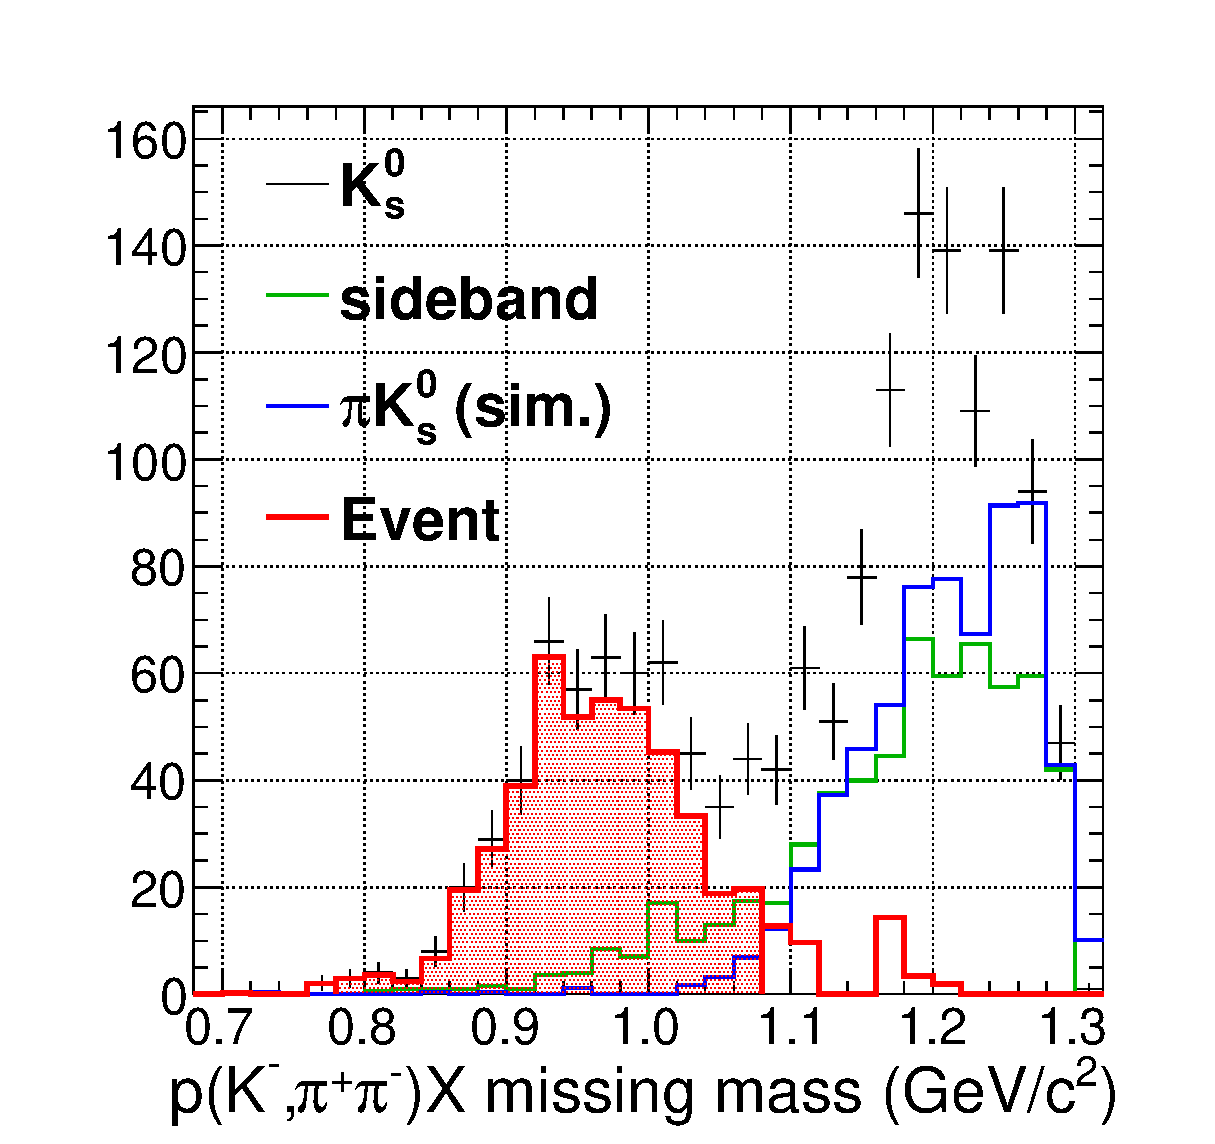
\includegraphics[width=\columnwidth]{./fig/nceff-missn.eps}
\end{center}
\end{minipage}
\begin{minipage}{0.5\textwidth}
\begin{center}
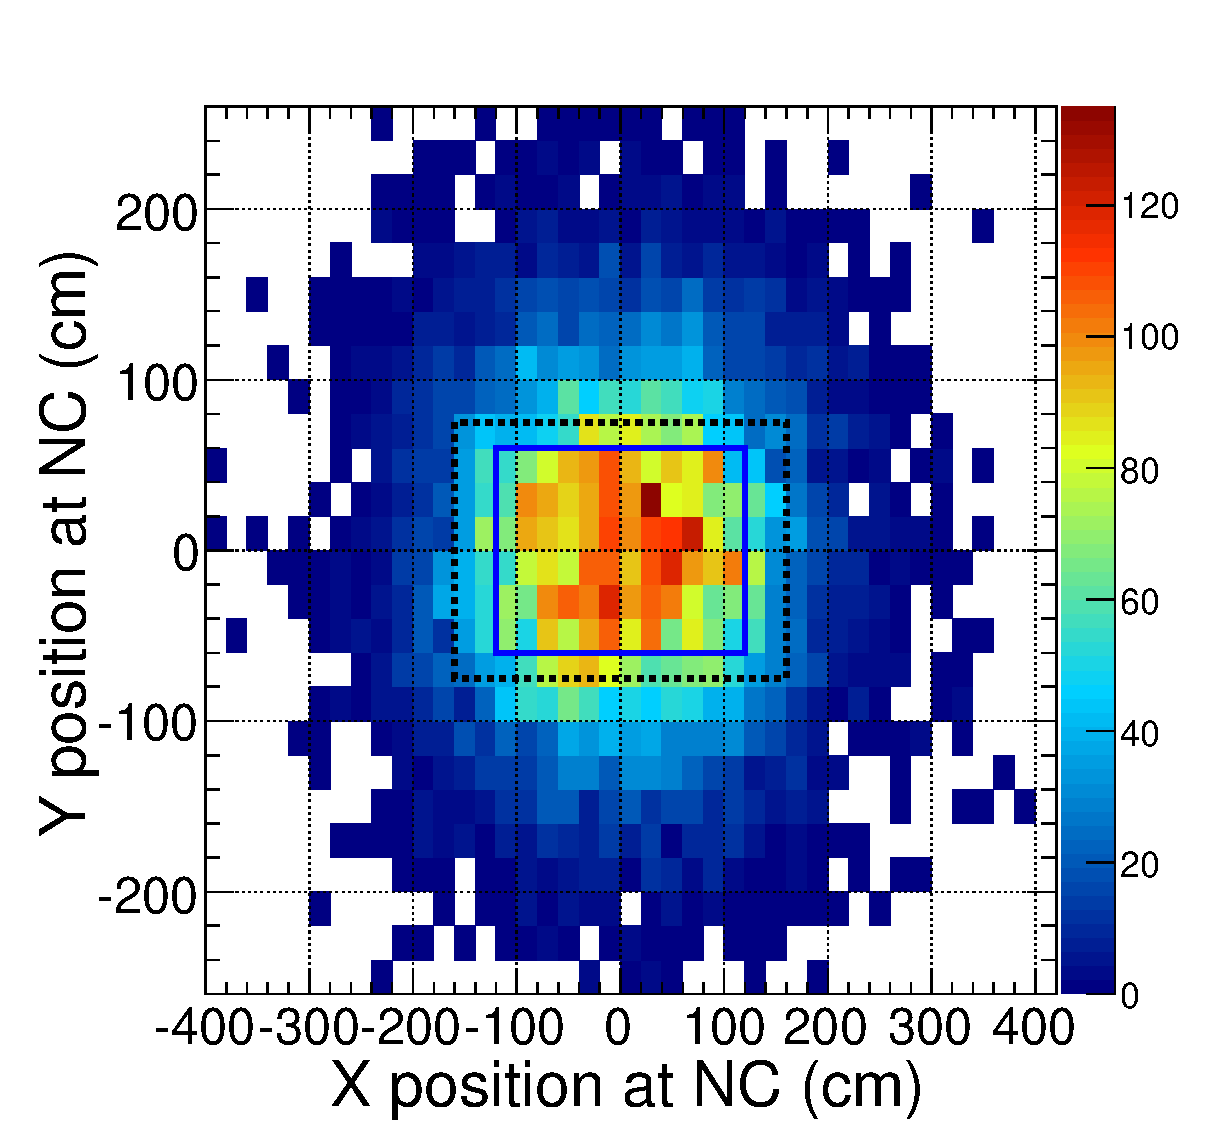
\includegraphics[width=\columnwidth]{./fig/nceff-posatnc.eps}
\end{center}
\end{minipage}
%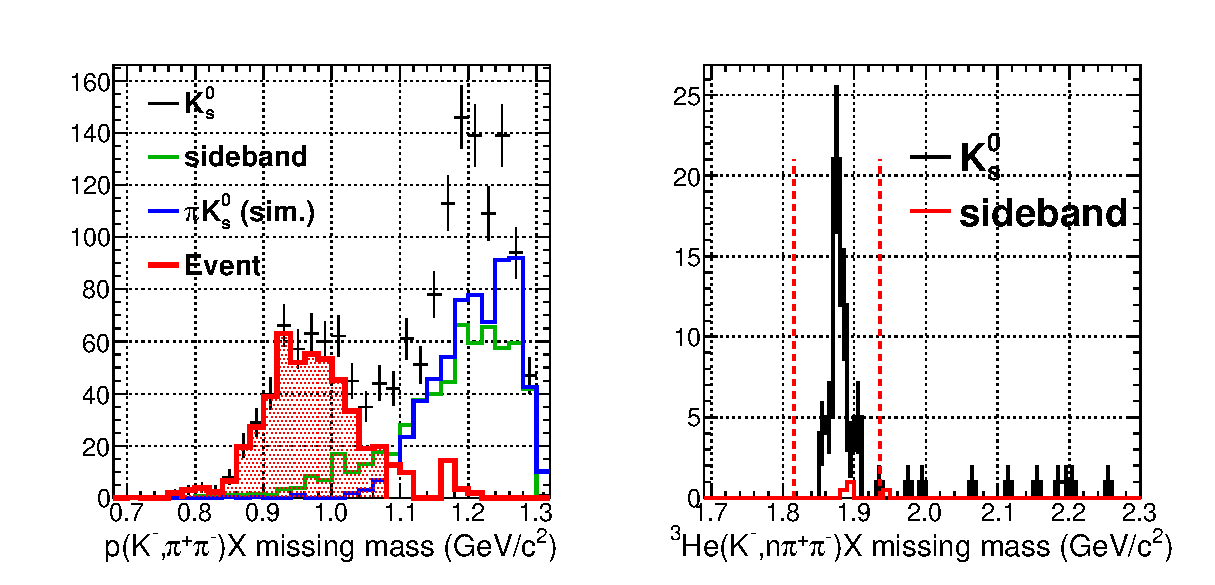
\includegraphics[width=\columnwidth]{./fig/nc-eff3.eps}
\caption[Decomposition of the p($K^-,\pi^+\pi^-$)X missing-mass spectrum and simulated position distribution of the neutron on the NC plane.]{(left) Typical decomposition of the p($K^-,\pi^+\pi^-$)X missing-mass spectrum. The red hatched area is selected as missing neutron event. (right) Simulated position distribution of the neutron on the NC plane when the missing momentum is extrapolated to inside the blue box. The back dotted box represents the NC size.}
\label{fig-nceff1}
\end{figure}  

\subsection{Trajectory of the missing neutron}
The expected NC hit-position can be obtained by extrapolating the missing momentum of $p(K^-,K^0_s)X$. However, we have a large uncertainty of the missing momentum of the neutron mainly due to the Fermi motion in $^3$He. We evaluated this effect by using the simulation, and obtained the position uncertainty of the extrapolated trajectory on the NC to be $\sim$ 1 m as shown in Fig. \ref{fig-nceff1}(right). With the simulation, the ratio of the NC incident events to the position-matched events, $R$, was also obtained for several regions on the NC defined in Fig. \ref{fig-nceff2}(left). Figure \ref{fig-nceff2}(right) shows the obtained ratio, where 10\% systematic error arise from the uncertainties in the missing-momentum resolution of the $p(K^-,K^0_s)X$ reaction and the contamination of ($p_s+n_s$) events.

\begin{figure}[]
\begin{minipage}{0.5\textwidth}
\begin{center}
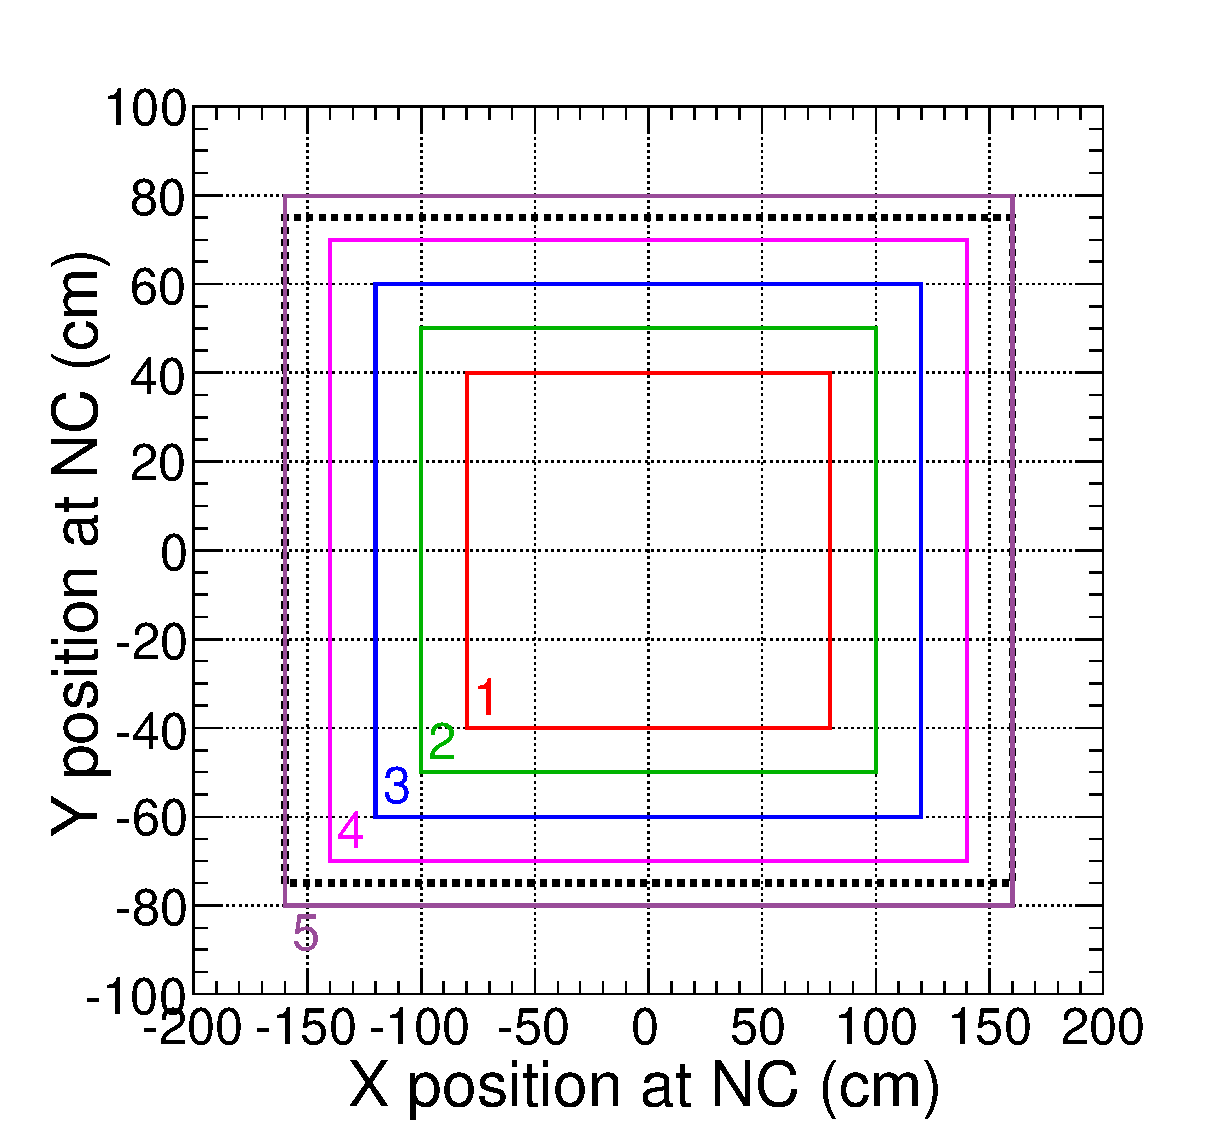
\includegraphics[width=\columnwidth]{./fig/nceff-ncregion.eps}
\end{center}
\end{minipage}
\begin{minipage}{0.5\textwidth}
\begin{center}
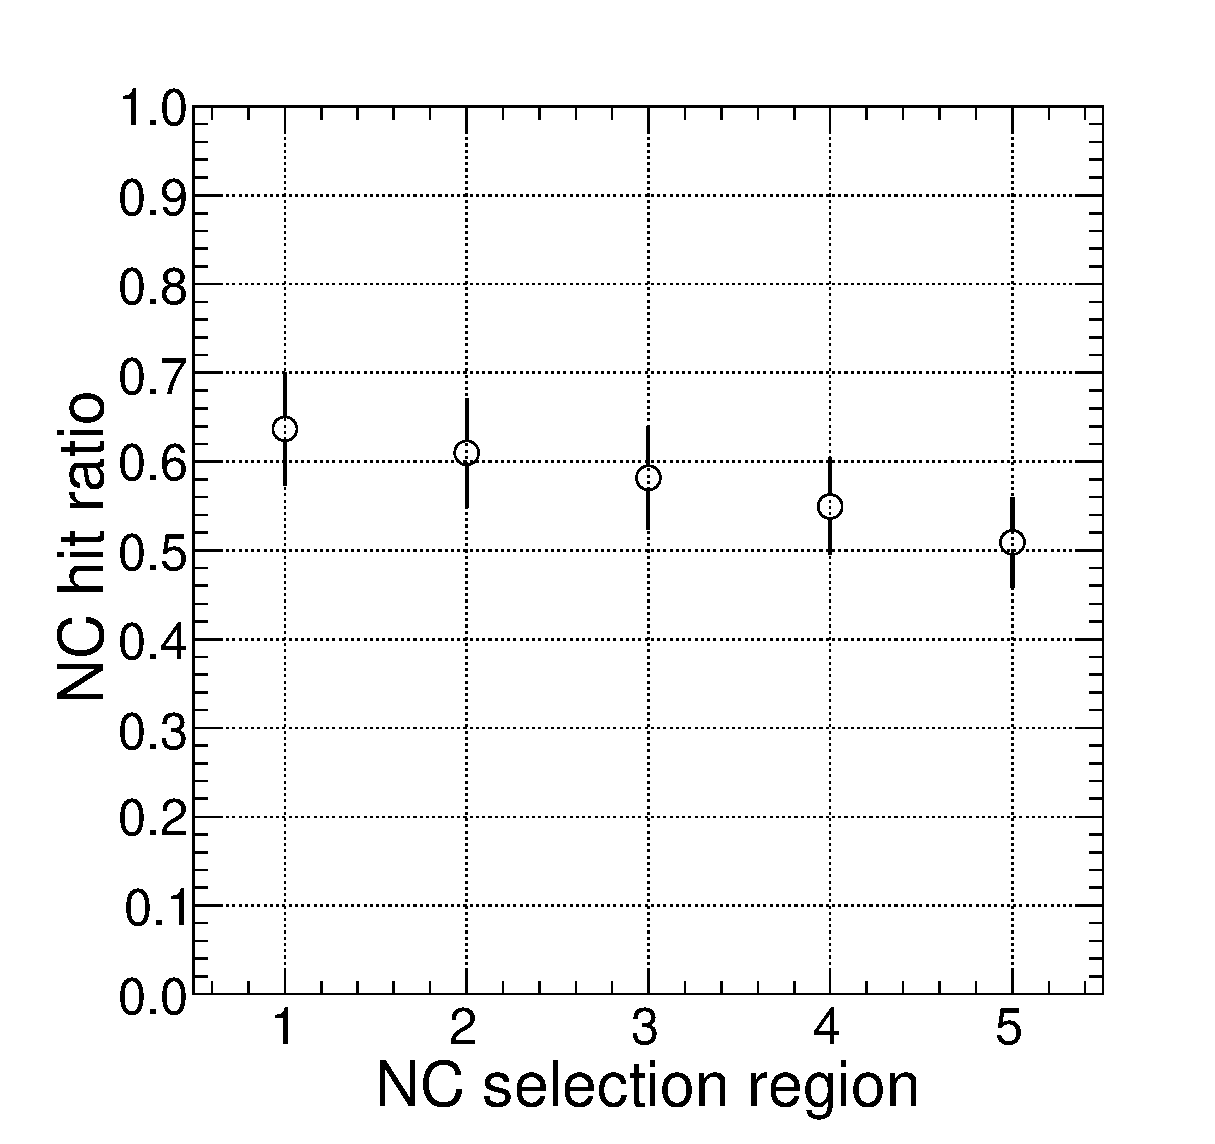
\includegraphics[width=\columnwidth]{./fig/nceff-ratio.eps}
\end{center}
\end{minipage}
%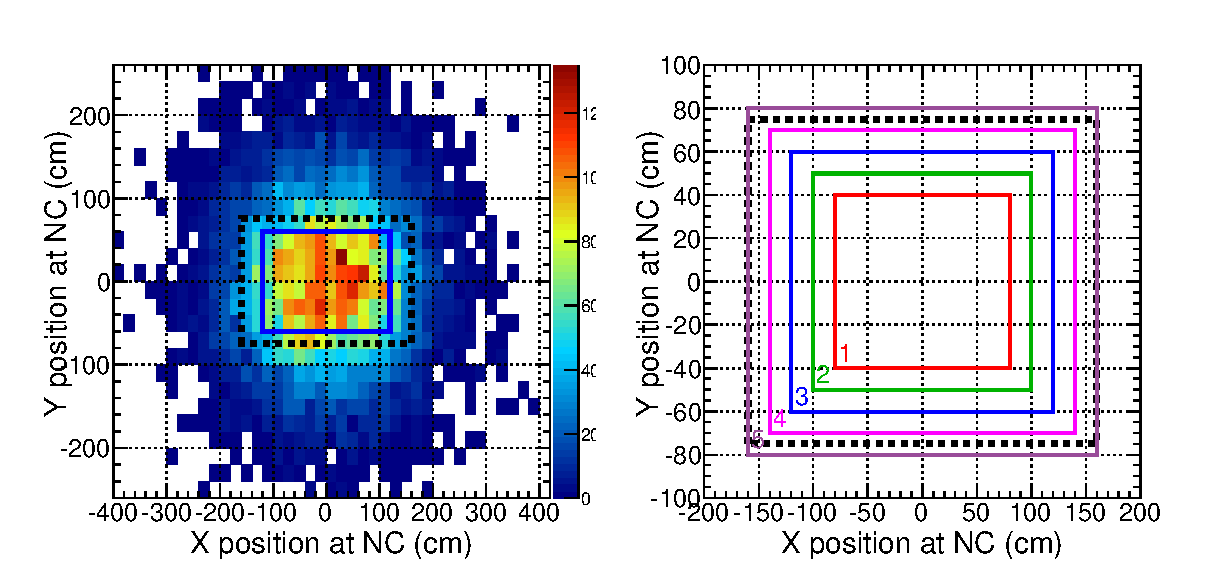
\includegraphics[width=\columnwidth]{./fig/nc-eff1.eps}
\caption[Definitions of the NC selection regions and simulated NC hit ratio $R$.]{(left) Definitions of the NC selection regions. (right) Simulated NC hit ratio $R$ when the missing momentum of the neutron is extrapolated to inside the defined region.}
\label{fig-nceff2}
\end{figure}  

\subsection{Selection of the NC signal}
The neutron associated in the reaction (\ref{eq-chargeex}) was identified by calculating a missing mass of $^3$He($K^-,nK^0_s$)X, where X should be a spectator deuteron. In the missing-mass distribution, a clear peak of the deuteron can be seen as shown in Figure \ref{fig-nceff3}(left). We selected the deuteron to subtract the contamination from the pion associated reactions in the neutron-detected events. 

\subsection{Detection efficiency}
Then the neutron detection efficiency of the NC can be evaluated with the event numbers obtained in above analysis procedure, \begin{eqnarray*}
\epsilon_{NC}&=&\frac{{\rm Number\ of\ fired\ neutron\ in\ the\ NC }}{{\rm Number\ of\ neutron\ on\ the\ NC}}\\
&=&\frac{N^{K^0_s}_{neutron}-N^{sideband}_{neutron}}{(N^{K^0_s}_{missN}-N^{sideband}_{missN}-N^{\pi K^0_s}_{missN})\times R \times \epsilon^{BVC\cup CVC}_{over\ veto}},
\end{eqnarray*}
where $N^{K^0_s}_{missN}$, $N^{sideband}_{missN}$, and $N^{\pi K^0_s}_{missN}$ are the numbers of the position-matched missing-neutron events in the $K^0_s$ region, the non-resonant background, and the pion associated reactions, respectively, and $N^{K^0_s}_{neutron}$ and $N^{sideband}_{neutron}$ are the number of the detected neutrons associated to the reaction \ref{eq-chargeex} in the the $K^0_s$ region and the non-resonant background, respectively. $\epsilon^{BVC\cup CVC}_{over\ veto}$ is the neutron over veto efficiency described in Sec. \ref{sec-overveto}.
The obtained efficiencies are stable against the NC selection regions as shown in Fig. \ref{fig-nceff3}(right). We adopted the average value in the NC selection 2$\sim$5 as the NC detection efficiency. Since the 4 values are not independent, the statistical error was determined conservatively by employing maximum one among the four. In addition, we evaluated the systematic error from the uncertainty in $R$. 
Then, the detection efficiency is
\begin{eqnarray*}
\epsilon_{NC}=0.23\pm 0.03(stat.) \pm 0.02(syst.).
\end{eqnarray*}

\begin{figure}[]
\begin{minipage}{0.5\textwidth}
\begin{center}
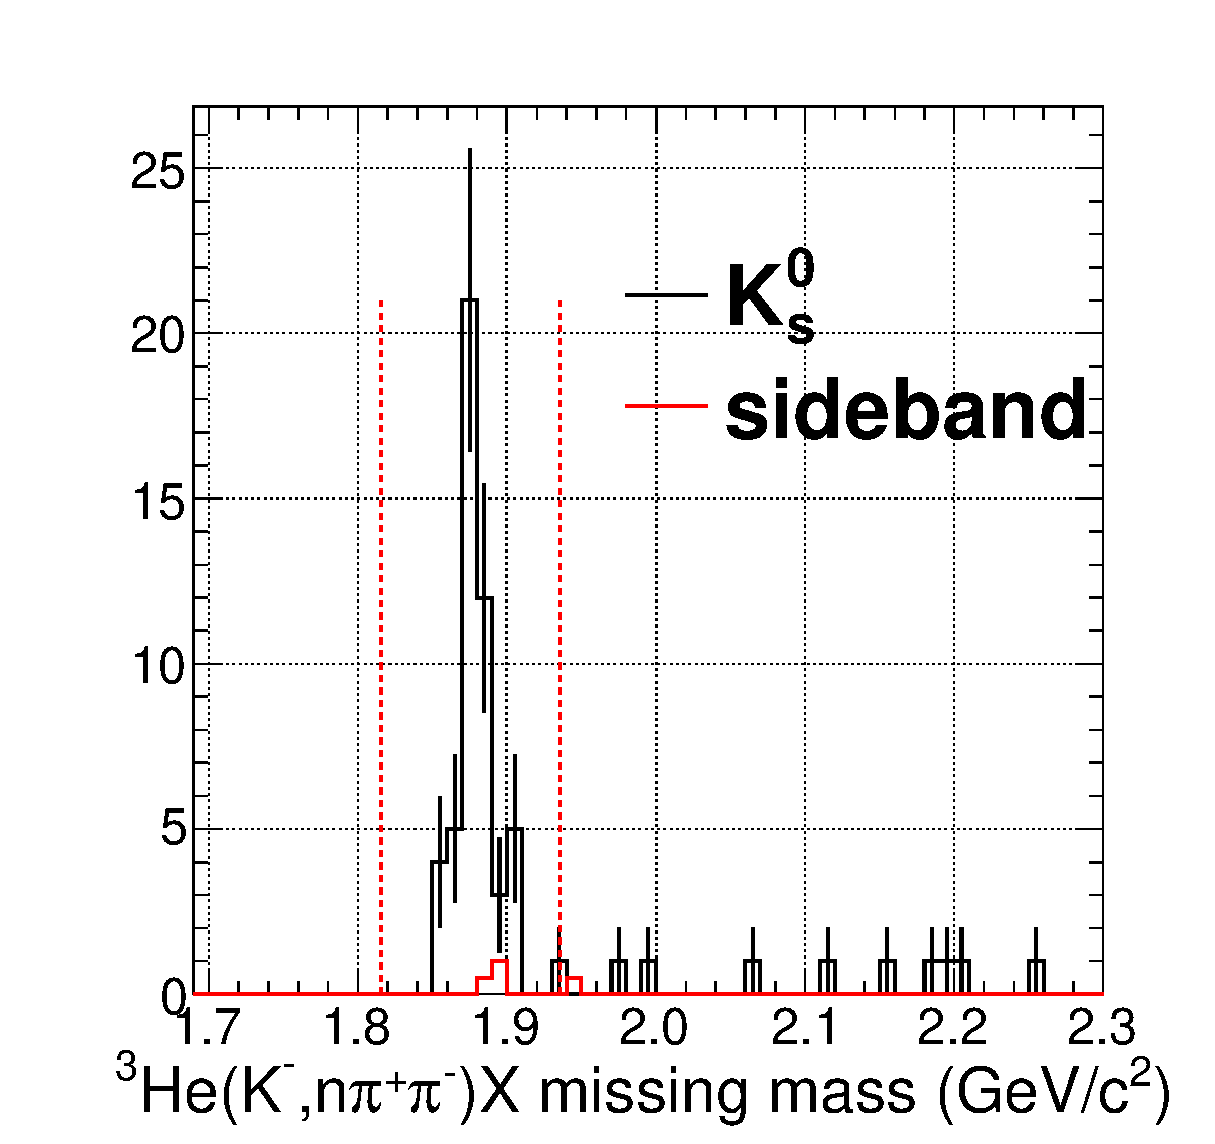
\includegraphics[width=\columnwidth]{./fig/nceff-missd.eps}
\end{center}
\end{minipage}
\begin{minipage}{0.5\textwidth}
\begin{center}
\includegraphics[width=\columnwidth]{./fig/nceff-result.eps}
\end{center}
\end{minipage}
\begin{center}
%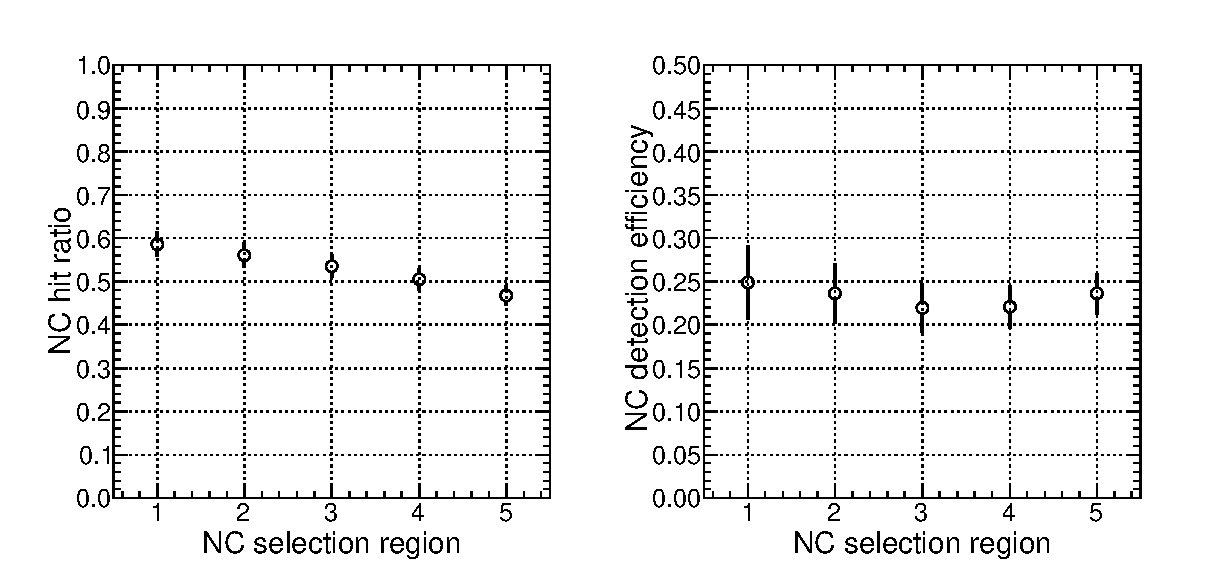
\includegraphics[width=\columnwidth]{./fig/nc-eff2.eps}
\caption[$^3$He($K^-,nK^0_s$)X missing mass spectrum and NC detection efficiency.]{(left) $^3$He($K^-,nK^0_s$)X missing-mass spectrum. Selection region of the missing deuteron is defined with the two red dotted lines. (right) NC detection efficiency for the NC selection regions.}
\label{fig-nceff3}
\end{center}
\end{figure}  

\section{Normalization factors for cross-section evaluation\label{sec-norm}}
The double differential cross section of the $^3$He($K^-,n$)X reaction is,
\begin{eqnarray}
\frac{dN}{dM}&=&\frac{d^2\sigma}{d\Omega dM}\cdot L \cdot \epsilon_{vertex} \cdot(1-f^n_{abs})\nonumber\\
& &\cdot \epsilon_{NC} \cdot (1-\epsilon_{over\ veto}^{BVC\cup CVC})  \cdot A_{NC} \cdot A_{CDS} \cdot\epsilon_{DAQ} \cdot \epsilon_{trig}, \label{eq-ncs}
%\frac{d^2N}{d\Omega dM}=\frac{d^2\sigma}{d\Omega dM}\cdot L \cdot \epsilon_{vertex} \cdot(1-f^n_{abs})\cdot \epsilon_{NC} \cdot A_{NC} \cdot A_{CDS} \cdot\epsilon_{DAQ} \cdot \epsilon_{trig}, \label{eq-ncs}
\end{eqnarray}
where $\frac{dN}{dM}$ is the observed missing mass distribution, $\epsilon_{vertex}$ is the vertex reconstruction efficiency with taking account of expected track number in the CDC, $\epsilon_{over\ veto}^{BVC\cup CVC}$ is the neutron over veto efficiency by the BVC and the CVC, $f^n_{abs}$ is a neutron absorption factor, $A_{NC}$ is the geometrical acceptance of the NC and $A_{CDS}$ is the CDS tagging acceptance, namely the probability of having at least one charged particle within the CDS acceptance. These factors are discussed in the following subsections. The integral luminosity $L$, the neutron detection efficiency $\epsilon_{NC}$, 
%the neutron over veto efficiency $\epsilon_{overveto}^n$, 
the live rate of the data acquisition system $\epsilon_{DAQ}$, and the trigger efficiency $\epsilon_{trig}$ are evaluated in Sec. \ref{sec-luminosity}, % Sec. \ref{}, 
Sec. \ref{sec-nceff}, Sec. \ref{sec-daqrate}, and Sec. \ref{sec-trigeff}, respectively.
 
Note that $A_{CDS}$ depends on the reaction channel, while other values are assumed to be common to all the reactions. 


\begin{table}[]
\caption{Summary of the normalization factors and the systematic uncertainties for the neutron yield.}
\begin{center}
\begin{tabular}{ll|cc} 
\hline\hline
		&	value	&	relative error (\%)			\\
\hline								
Luminosity $L$	($\mu$b$^{-1}$)	&	540	&	1.9			\\
$\epsilon_{vertex}$		&	0.98	&	2			\\
$1-f^n_{abs}$		&	0.946	&	1			\\
$\epsilon_{NC}$		&	0.23	&	16.5			\\
$1-\epsilon^{BVC\cup CVC}_{over\ veto}$		&	0.922	&	0.2			\\
$A_{NC}$	(msr)	&	22.1	&	1			\\
$\epsilon_{DAQ}$		&	0.815	&	0.9			\\
$\epsilon_{trig}$		&	0.983	&	0.1			\\
\hline								
total		&		&	16.9			\\
\hline\hline
\end{tabular}
\end{center}
\label{tab-ncs}
\end{table}%


\subsection{Neutron over veto efficiency\label{sec-overveto}}
Some neutron events were over vetoed by the BVC and/or the CVC mainly due to the accidental coincidence of the beam-pileup events. The over veto efficiency was evaluated using neutrons at the quasi-free peak, $\beta$=(1.25,1.3). The neutrons were identified with the NC only, where the first layer of the NC was used as the charged veto. The veto gate was set to (-10, 10) ns with respect to the quasi-free peak. Then, the event reduction rates were evaluated by applying vetoes with the BVC and/or the CVC. The obtained over veto efficiencies were,
\begin{eqnarray*}
\epsilon^{BVC}_{over\ veto}&=&4.9 \pm 0.2\%, \\
\epsilon^{CVC}_{over\ veto}&=&3.4 \pm 0.2\%, \\
\epsilon^{BVC\cup CVC}_{over\ veto}&=&7.8 \pm 0.2\%,
\end{eqnarray*}
where $\epsilon^{BVC}_{over\ veto}$, $\epsilon^{CVC}_{over\ veto}$, and $\epsilon^{BVC\cup CVC}_{over\ veto}$ are the over veto efficiency by the BVC, by the CVC, and by both the BVC and the CVC, respectively. The errors are statistical ones.

\subsection{Determination of threshold on the energy deposit}
Figure \ref{fig-ncbetade} shows the correlation between the energy deposit on the selected segment of the NC and $1/\beta$. Accidental events are concentrated in the small energy deposit region, while the fast neutrons give rather large energy deposit. Since reduction of the accidental background is essential to search for a tiny signal of the $K^-pp$ state, we studied the software threshold dependence of the energy deposit.

\subsection{Vertex reconstruction efficiency}
The vertex reconstruction efficiency was obtained by taking account of the track multiplicity in the CDS and the tracking efficiency of the CDC track. The vertex reconstruction efficiency $\epsilon_{vertex}$ was calculated as
\begin{eqnarray*}
\epsilon_{vertex} = \sum_{n=1}^6 R_n \cdot(1-(1-\epsilon_{CDC})^n),
\end{eqnarray*}
where $R_n$ is the ratio of the CDC track multiplicity n obtained from the track multiplicity distribution as shown in Fig. \ref{fig-cdcdca}(left), and $\epsilon_{CDC}$ is the tracking efficiency of the CDC evaluated in Sec. \ref{sec-cdceff}. The error was evaluated by propagating the error of $\epsilon_{CDC}$. The obtained efficiency is $\epsilon_{vertex}=0.98\pm0.02$. Although $R_n$ was underestimated by not taking into account the CDC tracking efficiecny, its effect to the obtained efficiency $\epsilon_{vertex}$ is negligibly small. 
\if0
\begin{figure}[]
\begin{center}
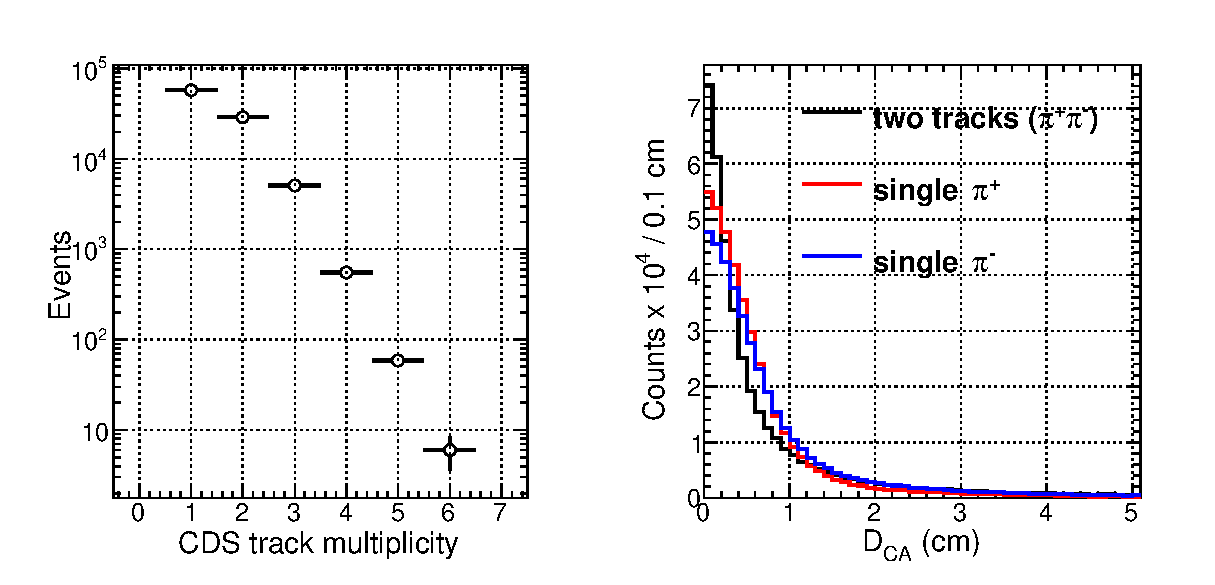
\includegraphics[width=9cm]{./fig/cdc-mul.eps}
\caption{Track multiplicity of the CDC with a requirement of a neutron in the NC.}
\label{fig-cdcmul}
\end{center}
\end{figure}  
\fi
\subsection{Neutron absorption between the target and the NC}
A small fraction of forward neutrons react with the materials between the target and the NC. Such neutrons are expected to be scattered out of the NC acceptance, or to produce charged particles to be vetoed. Therefore, they are not detected with the NC.

From the thickness of the NC ($\sim$36 g/cm$^2$) and the obtained NC detection efficiency, an effective attenuation coefficient of neutrons around 1 GeV/$c$ is estimated to be $\sim$125 g/cm$^2$. The total material thickness between the target and the NC is $\sim$7 g/cm$^2$ as summarized in Table \ref{tab-matforward}. Therefore, about 5\% neutrons are lost before the NC. The associated error was the same as that of the NC detection efficiency. Note that the difference of the reaction cross section in the different materials was not considered in this evaluation.

\subsection{NC geometrical Acceptance}
The geometrical acceptance of the NC was obtained to be 22.1 msr with the NC size of 3.2 m (horizontal)  $\times$ 1.5 m (vertical) and the distance of 14.73 m between the center of the fiducial volume and the first layer of the NC. The uncertainty due to the vertex distribution in the fiducial volume was evaluated to be 1\% at maximum.

\subsection{Summary of the systematical uncertainty}
We evaluated the systematic uncertainty in the missing mass scale to be 3 MeV/$c^2$ as described in Sec. \ref{sec-scale}. As for the systematic uncertainty of the neutron yield from the $^3$He($K^-,n$) reaction, a quadratic sum of the errors associated to Eq. (\ref{eq-ncs}) was adopted. The calculated value is 16.8\%, where the uncertainty of the NC detection efficiency is dominant. The normalization factors and the systematic uncertainties for the neutron yield are summarized in Table \ref{tab-ncs}. 

